\begin{frame}
\frametitle{Chemical removal rates have a small impact in the 0D scaled model}
\begin{columns}
    \column[t]{0.45\textwidth}
    \begin{block}{Group half-lives:}
        \begin{figure}[!ht]
            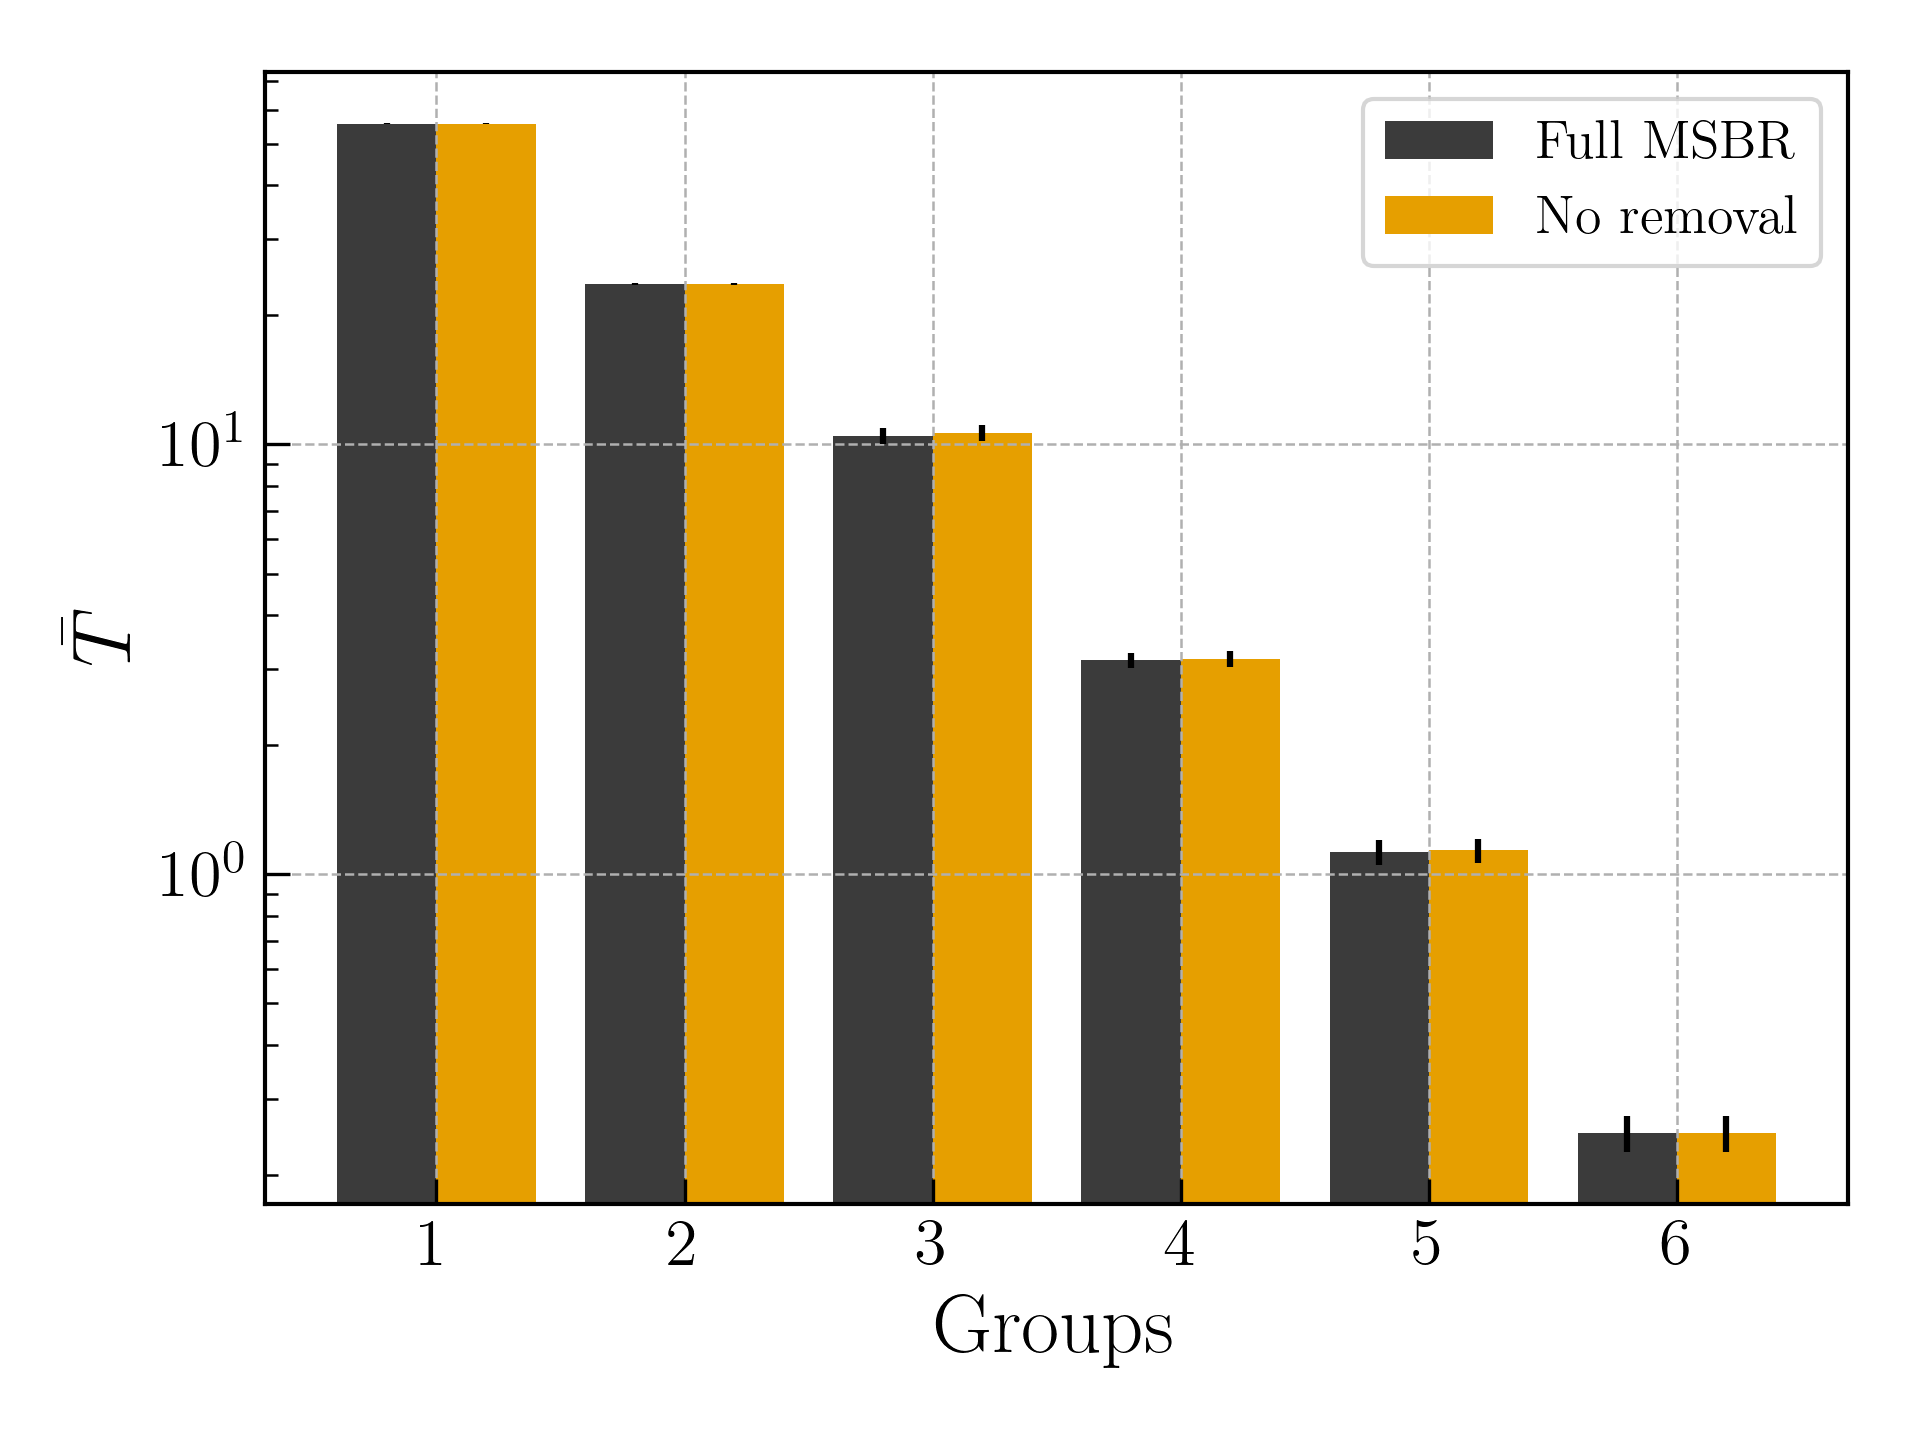
\includegraphics[width=1.0\linewidth]{../images/halflives_chem_bool.png} 
            \caption{$\tau_k$ for each \gls{DNP} group $k$ after a thermal saturation irradiation of $^{235}$U using the 0D scaled model.}
        \end{figure} 
    \end{block}
    \column[t]{0.45\textwidth}
    \begin{block}{Group yields:}
        \begin{figure}[!ht]
            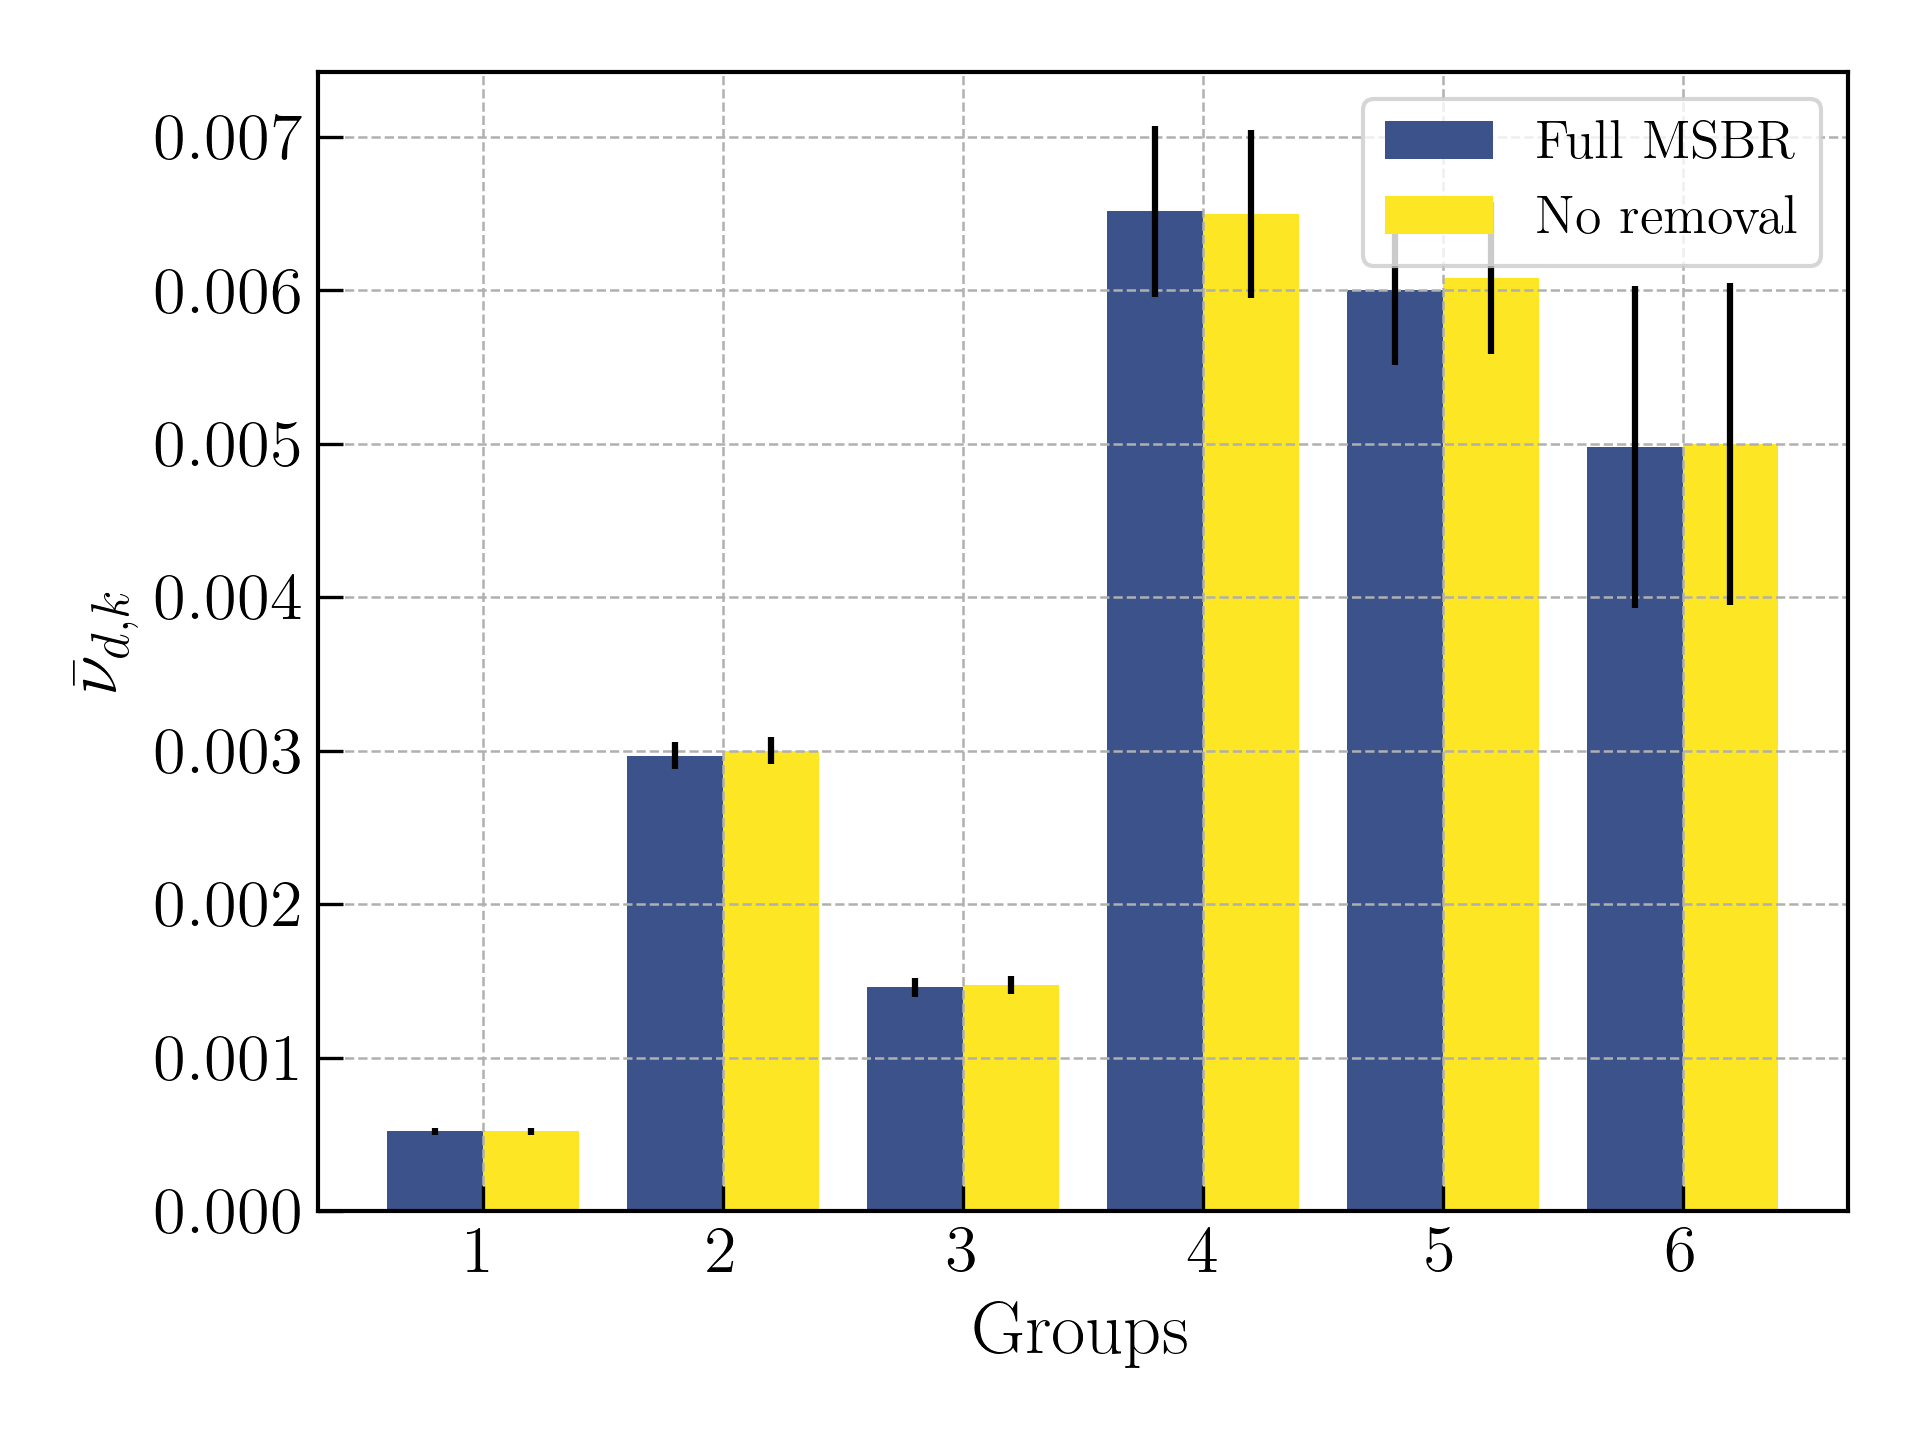
\includegraphics[width=1.0\linewidth]{../images/yields_chem_bool.png} 
            \caption{$\bar{\nu}_{d,k}$ for each \gls{DNP} group $k$ after a thermal saturation irradiation of $^{235}$U using the 0D scaled model.}
        \end{figure} 
    \end{block}
\end{columns}
\textbf{The differences induced by exclusion of removal rates with cycle times longer than 20 seconds are minimal and well within uncertainty bounds.Neglecting chemical removal rates generally leads to larger yields, though all differences are within uncertainty bounds.}

\end{frame}